\documentclass{ximera}

%\usepackage{todonotes}

\newcommand{\todo}{}

\usepackage{esint} % for \oiint
\ifxake%%https://math.meta.stackexchange.com/questions/9973/how-do-you-render-a-closed-surface-double-integral
\renewcommand{\oiint}{{\large\bigcirc}\kern-1.56em\iint}
\fi


\graphicspath{
  {./}
  {ximeraTutorial/}
  {basicPhilosophy/}
  {functionsOfSeveralVariables/}
  {normalVectors/}
  {lagrangeMultipliers/}
  {vectorFields/}
  {greensTheorem/}
  {shapeOfThingsToCome/}
  {dotProducts/}
  {partialDerivativesAndTheGradientVector/}
  {../productAndQuotientRules/exercises/}
  {../normalVectors/exercisesParametricPlots/}
  {../continuityOfFunctionsOfSeveralVariables/exercises/}
  {../partialDerivativesAndTheGradientVector/exercises/}
  {../directionalDerivativeAndChainRule/exercises/}
  {../commonCoordinates/exercisesCylindricalCoordinates/}
  {../commonCoordinates/exercisesSphericalCoordinates/}
  {../greensTheorem/exercisesCurlAndLineIntegrals/}
  {../greensTheorem/exercisesDivergenceAndLineIntegrals/}
  {../shapeOfThingsToCome/exercisesDivergenceTheorem/}
  {../greensTheorem/}
  {../shapeOfThingsToCome/}
  {../separableDifferentialEquations/exercises/}
  {vectorFields/}
}

\newcommand{\mooculus}{\textsf{\textbf{MOOC}\textnormal{\textsf{ULUS}}}}

\usepackage{tkz-euclide}
\usepackage{tikz}
\usepackage{tikz-cd}
\usetikzlibrary{arrows}
\tikzset{>=stealth,commutative diagrams/.cd,
  arrow style=tikz,diagrams={>=stealth}} %% cool arrow head
\tikzset{shorten <>/.style={ shorten >=#1, shorten <=#1 } } %% allows shorter vectors

\usetikzlibrary{backgrounds} %% for boxes around graphs
\usetikzlibrary{shapes,positioning}  %% Clouds and stars
\usetikzlibrary{matrix} %% for matrix
\usepgfplotslibrary{polar} %% for polar plots
\usepgfplotslibrary{fillbetween} %% to shade area between curves in TikZ
%\usetkzobj{all}
\usepackage[makeroom]{cancel} %% for strike outs
%\usepackage{mathtools} %% for pretty underbrace % Breaks Ximera
%\usepackage{multicol}
\usepackage{pgffor} %% required for integral for loops



%% http://tex.stackexchange.com/questions/66490/drawing-a-tikz-arc-specifying-the-center
%% Draws beach ball
\tikzset{pics/carc/.style args={#1:#2:#3}{code={\draw[pic actions] (#1:#3) arc(#1:#2:#3);}}}



\usepackage{array}
\setlength{\extrarowheight}{+.1cm}
\newdimen\digitwidth
\settowidth\digitwidth{9}
\def\divrule#1#2{
\noalign{\moveright#1\digitwidth
\vbox{\hrule width#2\digitwidth}}}




% \newcommand{\RR}{\mathbb R}
% \newcommand{\R}{\mathbb R}
% \newcommand{\N}{\mathbb N}
% \newcommand{\Z}{\mathbb Z}

\newcommand{\sagemath}{\textsf{SageMath}}


%\renewcommand{\d}{\,d\!}
%\renewcommand{\d}{\mathop{}\!d}
%\newcommand{\dd}[2][]{\frac{\d #1}{\d #2}}
%\newcommand{\pp}[2][]{\frac{\partial #1}{\partial #2}}
% \renewcommand{\l}{\ell}
%\newcommand{\ddx}{\frac{d}{\d x}}

% \newcommand{\zeroOverZero}{\ensuremath{\boldsymbol{\tfrac{0}{0}}}}
%\newcommand{\inftyOverInfty}{\ensuremath{\boldsymbol{\tfrac{\infty}{\infty}}}}
%\newcommand{\zeroOverInfty}{\ensuremath{\boldsymbol{\tfrac{0}{\infty}}}}
%\newcommand{\zeroTimesInfty}{\ensuremath{\small\boldsymbol{0\cdot \infty}}}
%\newcommand{\inftyMinusInfty}{\ensuremath{\small\boldsymbol{\infty - \infty}}}
%\newcommand{\oneToInfty}{\ensuremath{\boldsymbol{1^\infty}}}
%\newcommand{\zeroToZero}{\ensuremath{\boldsymbol{0^0}}}
%\newcommand{\inftyToZero}{\ensuremath{\boldsymbol{\infty^0}}}



% \newcommand{\numOverZero}{\ensuremath{\boldsymbol{\tfrac{\#}{0}}}}
% \newcommand{\dfn}{\textbf}
% \newcommand{\unit}{\,\mathrm}
% \newcommand{\unit}{\mathop{}\!\mathrm}
% \newcommand{\eval}[1]{\bigg[ #1 \bigg]}
% \newcommand{\seq}[1]{\left( #1 \right)}
% \renewcommand{\epsilon}{\varepsilon}
% \renewcommand{\phi}{\varphi}


% \renewcommand{\iff}{\Leftrightarrow}

% \DeclareMathOperator{\arccot}{arccot}
% \DeclareMathOperator{\arcsec}{arcsec}
% \DeclareMathOperator{\arccsc}{arccsc}
% \DeclareMathOperator{\si}{Si}
% \DeclareMathOperator{\scal}{scal}
% \DeclareMathOperator{\sign}{sign}


%% \newcommand{\tightoverset}[2]{% for arrow vec
%%   \mathop{#2}\limits^{\vbox to -.5ex{\kern-0.75ex\hbox{$#1$}\vss}}}
% \newcommand{\arrowvec}[1]{{\overset{\rightharpoonup}{#1}}}
% \renewcommand{\vec}[1]{\arrowvec{\mathbf{#1}}}
% \renewcommand{\vec}[1]{{\overset{\boldsymbol{\rightharpoonup}}{\mathbf{#1}}}}

% \newcommand{\point}[1]{\left(#1\right)} %this allows \vector{ to be changed to \vector{ with a quick find and replace
% \newcommand{\pt}[1]{\mathbf{#1}} %this allows \vec{ to be changed to \vec{ with a quick find and replace
% \newcommand{\Lim}[2]{\lim_{\point{#1} \to \point{#2}}} %Bart, I changed this to point since I want to use it.  It runs through both of the exercise and exerciseE files in limits section, which is why it was in each document to start with.

% \DeclareMathOperator{\proj}{\mathbf{proj}}
% \newcommand{\veci}{{\boldsymbol{\hat{\imath}}}}
% \newcommand{\vecj}{{\boldsymbol{\hat{\jmath}}}}
% \newcommand{\veck}{{\boldsymbol{\hat{k}}}}
% \newcommand{\vecl}{\vec{\boldsymbol{\l}}}
% \newcommand{\uvec}[1]{\mathbf{\hat{#1}}}
% \newcommand{\utan}{\mathbf{\hat{t}}}
% \newcommand{\unormal}{\mathbf{\hat{n}}}
% \newcommand{\ubinormal}{\mathbf{\hat{b}}}

% \newcommand{\dotp}{\bullet}
% \newcommand{\cross}{\boldsymbol\times}
% \newcommand{\grad}{\boldsymbol\nabla}
% \newcommand{\divergence}{\grad\dotp}
% \newcommand{\curl}{\grad\cross}
%\DeclareMathOperator{\divergence}{divergence}
%\DeclareMathOperator{\curl}[1]{\grad\cross #1}
% \newcommand{\lto}{\mathop{\longrightarrow\,}\limits}

% \renewcommand{\bar}{\overline}

\colorlet{textColor}{black}
\colorlet{background}{white}
\colorlet{penColor}{blue!50!black} % Color of a curve in a plot
\colorlet{penColor2}{red!50!black}% Color of a curve in a plot
\colorlet{penColor3}{red!50!blue} % Color of a curve in a plot
\colorlet{penColor4}{green!50!black} % Color of a curve in a plot
\colorlet{penColor5}{orange!80!black} % Color of a curve in a plot
\colorlet{penColor6}{yellow!70!black} % Color of a curve in a plot
\colorlet{fill1}{penColor!20} % Color of fill in a plot
\colorlet{fill2}{penColor2!20} % Color of fill in a plot
\colorlet{fillp}{fill1} % Color of positive area
\colorlet{filln}{penColor2!20} % Color of negative area
\colorlet{fill3}{penColor3!20} % Fill
\colorlet{fill4}{penColor4!20} % Fill
\colorlet{fill5}{penColor5!20} % Fill
\colorlet{gridColor}{gray!50} % Color of grid in a plot

\newcommand{\surfaceColor}{violet}
\newcommand{\surfaceColorTwo}{redyellow}
\newcommand{\sliceColor}{greenyellow}




\pgfmathdeclarefunction{gauss}{2}{% gives gaussian
  \pgfmathparse{1/(#2*sqrt(2*pi))*exp(-((x-#1)^2)/(2*#2^2))}%
}


%%%%%%%%%%%%%
%% Vectors
%%%%%%%%%%%%%

%% Simple horiz vectors
\renewcommand{\vector}[1]{\left\langle #1\right\rangle}


%% %% Complex Horiz Vectors with angle brackets
%% \makeatletter
%% \renewcommand{\vector}[2][ , ]{\left\langle%
%%   \def\nextitem{\def\nextitem{#1}}%
%%   \@for \el:=#2\do{\nextitem\el}\right\rangle%
%% }
%% \makeatother

%% %% Vertical Vectors
%% \def\vector#1{\begin{bmatrix}\vecListA#1,,\end{bmatrix}}
%% \def\vecListA#1,{\if,#1,\else #1\cr \expandafter \vecListA \fi}

%%%%%%%%%%%%%
%% End of vectors
%%%%%%%%%%%%%

%\newcommand{\fullwidth}{}
%\newcommand{\normalwidth}{}



%% makes a snazzy t-chart for evaluating functions
%\newenvironment{tchart}{\rowcolors{2}{}{background!90!textColor}\array}{\endarray}

%%This is to help with formatting on future title pages.
\newenvironment{sectionOutcomes}{}{}



%% Flowchart stuff
%\tikzstyle{startstop} = [rectangle, rounded corners, minimum width=3cm, minimum height=1cm,text centered, draw=black]
%\tikzstyle{question} = [rectangle, minimum width=3cm, minimum height=1cm, text centered, draw=black]
%\tikzstyle{decision} = [trapezium, trapezium left angle=70, trapezium right angle=110, minimum width=3cm, minimum height=1cm, text centered, draw=black]
%\tikzstyle{question} = [rectangle, rounded corners, minimum width=3cm, minimum height=1cm,text centered, draw=black]
%\tikzstyle{process} = [rectangle, minimum width=3cm, minimum height=1cm, text centered, draw=black]
%\tikzstyle{decision} = [trapezium, trapezium left angle=70, trapezium right angle=110, minimum width=3cm, minimum height=1cm, text centered, draw=black]

\author{Bart Snapp and Jim Talamo (edited)}

\outcome{Recognize sequences can be generated by functions.}
\outcome{Compute limits of sequences.}
\outcome{Understand growth rates of basic sequences.}
\outcome{Introduce important terminology for sequences.}
\outcome{Apply the monotone convergence theorem.}

\title{Limits of Sequences}

\begin{document}
\begin{abstract}
convergence
\end{abstract}
\maketitle

In the previous section, we defined a sequence as a function defined on a subset of the whole numbers, and we discussed how we can represent this by an ordered list.  We chose the notation $\{a_n\}_{n=1}$ to denote the list below.

\[
a_1, a_2, a_3 , \ldots
\]

In the previous section, we found many ways to generate this list.  Regardless of how we obtain it, there are two fundamental questions we can ask.
\begin{itemize}
\item[1.] Do the numbers in the list approach a finite value?
\item[2.] If so, what is that value?
\end{itemize}


We begin with an intuitive definition. \\

\begin{definition}\index{limit of a sequence}  \textbf{\textcolor{green!50!black}{Intuitive Limit}} 


  Given a sequence $\{a_n\}_{n =n_0}$, we say that the \textbf{limit} of the sequence is $L$ if, as $n$ grows arbitrarily large, $a_n$ becomes arbitrarily close to $L$. 
  
If $\lim\limits_{n\to\infty}a_n=L$ we say that the sequence
\textbf{converges}\index{convergent sequence}\index{sequence!convergent}.
If there is no finite value $L$ so that $\lim\limits_{n\to\infty}a_n = L$,
then we say that the limit \textbf{does not exist}, or equivalently that
the sequence \textbf{diverges}\index{divergent
  sequence}\index{sequence!divergent}.
\end{definition}

This intuitive definition of a limit can be made more precise as follows.

\begin{definition}\index{formal limit of a sequence}   \textbf{\textcolor{green!50!black}{Formal Limit}}   

\label{definition:limit-of-a-sequence}
Suppose that $\{a_n\}_{n=n_0}$ is a sequence.  We say that
$\lim\limits_{n\to \infty}a_n=L$ if for every $\epsilon>0$, there exists an integer $N$, such that $|a_n-L|<\epsilon$ for any $n \geq N$.
\end{definition}

This precise definition captures the same idea as the intuitive definition but makes it more precise.  The quantity $\epsilon$ measures how close the terms in the sequence are to the limit $L$.  We say that the limit exists and is $L$ if we can choose any distance we want the terms to be from $L$ and we know the terms in the sequence eventually become and stay that close to $L$.  

\begin{remark}
The precise definition is extremely important to establish the theoretical foundations of sequences and is used frequently in more theoretically-oriented courses.  For our purposes, however, the intuitive definition will be sufficient.
\end{remark}

\begin{question}
Suppose that $\{a_n\}_{n=1}$ is a sequence and that $\lim\limits_{n \to \infty} a_n = L$.  Intuitively, what can we say about $\lim\limits_{n \to \infty} a_{n+1}$? 


\begin{multipleChoice}
\choice {$\lim\limits_{n \to \infty} a_{n+1}$ exists, but we do not know what its value is.}
\choice [correct]{$\lim\limits_{n \to \infty} a_{n+1}$ exists, and $\lim\limits_{n \to \infty} a_{n+1}=L$ exists.}
\choice {$\lim\limits_{n \to \infty} a_{n+1}$ may or may not exist.}
\end{multipleChoice}




One way to think about this is by noting that the sequence $\{a_n\}_{n=1}$ is represented by the list

\[
a_1,a_2,a_3, \ldots ,
\]

while the sequence $\{a_{n+1}\}_{n=1}$ is represented by the list below.

\[
a_2,a_3,a_4, \ldots
\]

If the first sequence tends to $L$, the second sequence must also tend to $L$.

\end{question}




\begin{warning}
  In the case that $\lim\limits_{n \to \infty} a_n = \pm\infty$, we say that
  $\{a_n\}$ diverges.  The only time we say that a sequence converges
    is when the limit exists and is equal to a \textit{finite} value.
\end{warning}

%\youtube{https://www.youtube.com/watch?v=0UCRZAsIkXM}















\section*{Connections to real-valued functions}
Since sequences are functions defined on the integers, the notion of a ``limit at a specific $n$'' is not very interesting since we can explicitly find $a_n$ for a given $n$. However, limits at \textit{infinity} are a different story.  An important question can now be asked; given a sequence, how do we determine if it has a limit?  

There are several techniques that allow us to find limits of real-valued functions, and we have seen that if we have a sequence, we can often find a real-valued function that agrees with it on their common domains.   Suppose that we have found a real-valued function $f(x)$ that agrees with $a_n$ on their common domains, i.e. that $f(n)=a_n$.  If we know  $\lim\limits_{x\to\infty} f(x)$, can we use this to conclude something about $\lim\limits_{n \to \infty} a_n$?  

Before answering this question, consider the following cautionary example.

\begin{example}
  Let $a_n = \sin(n\pi)$ and $f(x) = \sin(\pi x)$. Show that
  \[
  \lim\limits_{n\to\infty} a_n \ne \lim\limits_{x\to \infty}f(x).
  \]
  \begin{explanation}
  The sequence $\{a_n\}_{n=1}^{\infty}$ is represented by the ordered  list of numbers below.
  \[
  \sin(0\pi),\, \sin(1\pi),\, \sin(2\pi),\,\sin(3\pi),\,\ldots
  \]
Since $\sin(n\pi)=0$, this list is actually a list of zeroes.
  \[
  0,\, 0 , \, 0 ,\,0,\,\ldots
  \]
Since every term in the sequence is $0$, we have
\[
\lim\limits_{n\to\infty} a_n = 0. 
\]
But $\lim\limits_{x\to\infty}f(x)$, when $x$ is real, does not exist; as $x$
becomes arbitrarily large, the values $\sin(x\pi)$ do not get closer and
closer to a single value, but instead oscillate between $-1$ and $1$.

This is shown graphically below.

\begin{image}
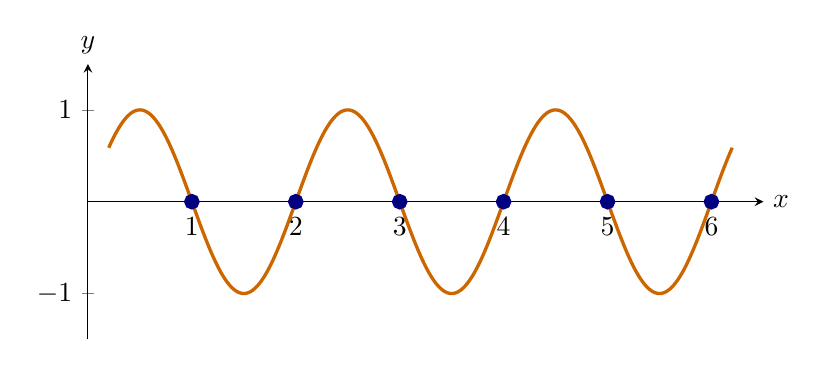
\begin{tikzpicture}
	\begin{axis}[
            domain=.8:6.5,xmin=0,xmax=6.5,ymin=-1.5,ymax=1.5,
            width=4in,
            height=2in,
            axis lines =middle, xlabel=$x$, ylabel=$y$,
            xtick={1,2,...,6},
            ytick={-1,1},
            every axis y label/.style={at=(current axis.above origin),anchor=south},
            every axis x label/.style={at=(current axis.right of origin),anchor=west},
            clip=false,
            %axis on top,
          ]
       
          \addplot [penColor5,very thick,smooth,domain=.2:6.2,samples=300]{sin(deg(pi*x)))};
          \addplot[color=penColor,fill=penColor,only marks,mark=*,ultra thick] coordinates{(1,0)};  %% closed hole        
          \addplot[color=penColor,fill=penColor,only marks,mark=*,ultra thick] coordinates{(2,0)};  %% closed hole        
          \addplot[color=penColor,fill=penColor,only marks,mark=*,ultra thick] coordinates{(3,0)};  %% closed hole        
          \addplot[color=penColor,fill=penColor,only marks,mark=*,ultra thick] coordinates{(4,0)};  %% closed hole        
          \addplot[color=penColor,fill=penColor,only marks,mark=*,ultra thick] coordinates{(5,0)};  %% closed hole    
          \addplot[color=penColor,fill=penColor,only marks,mark=*,ultra thick] coordinates{(6,0)};  %% closed hole         
        \end{axis}
\end{tikzpicture}
\end{image}


  \end{explanation}
\end{example}

What can we conclude from the above example?

\begin{multipleChoice}
\choice{If $\lim\limits_{n \to \infty} a_n$ exists, then $\lim\limits_{x \to \infty} f(x)$ exists.}
\choice{If  $\lim\limits_{x \to \infty} f(x)$ does not exist, then $\lim\limits_{n \to \infty} a_n$ does not exist.}
\choice[correct]{If $\lim\limits_{x \to \infty} f(x)$ does not exist, $\lim\limits_{n \to \infty} a_n$ may still exist.}
\end{multipleChoice}

This might lead us to believe that we need to develop a whole new arsenal of techniques in order to determine if limits of sequences exist, but there is good news.










\section*{Calculating limits of sequences}

\begin{theorem}
  Let $\{a_n\}$ be a sequence and suppose that $f(x)$ is a real-valued function for which $f(n) = a_n$ for all integers $n$.  If
  \[
  \text{If} \, \lim\limits_{x\to\infty}f(x)=L, \, \text{ then } \, \lim\limits_{n\to\infty} a_n=L \, \text{ as well. }
  \]
 
\end{theorem}

If we think about the theorem a bit further, the conclusion  of the theorem and the content of the preceding example should seem reasonable.  If the values of $f(x)$ become arbitrarily close to a number $L$ for \emph{all} arbitrarily large $x$-values, then the result should still hold when we only consider \emph{some} of these values.  However, if we only know what happens for \emph{some} arbitrarily large $x$-values, we cannot say what happens for \emph{all} of them!










\begin{example}
Let $a_n = \frac{5n+1}{6n+7}$.  Determine if the sequence $\{a_n\}_{n=1}^{\infty}$ has a limit.

\begin{explanation}
A function that can be used to generate the sequence is $f(x) = \frac{5x+1}{6x+7}$.  \\

Since $\lim\limits_{x \to \infty} \frac{5x+1}{6x+7} = \answer[given]{\frac{5}{6}}$, $\lim\limits_{n \to \infty} a_n = \answer[given]{\frac{5}{6}}$.
\end{explanation}

\end{example}







\begin{warning}
Remember that the converse of this theorem is not
true.  In the example preceding this theorem, we have an explicit example of a function $f(x)$ and a sequence $(a_n)$ where $a_n
=f(n)$ and
\[
\lim\limits_{x\to\infty}f(x)=\text{DNE} \quad\text{but} \quad \lim\limits_{n\to\infty} a_n = 0.
\]
\end{warning}

In practice, we use the above theorem to compute limits without explicitly exhibiting the function of a real variable from which the limit is derived.  










\begin{center}
\textbf{\textcolor{green!50!black}{ooooo-=-=-=-ooOoo-=-=-=-ooooo}} \\

more examples can be found by following this link\\ \link[More Examples of Limits of Sequences]{https://ximera.osu.edu/csccmathematics/precalculus2/precalculus2/limitOfSequences/examples/exampleList}

\end{center}






\end{document}
